\documentclass[12pt,a4paper]{article}
\linespread{1.0}
% Language setting
% Replace `english' with e.g. `spanish' to change the document language
\usepackage[english]{babel}
\usepackage[colorlinks,linkcolor=blue]{hyperref}
% Set page size and margins
% Replace `letterpaper' with `a4paper' for UK/EU standard size
\usepackage[letterpaper,top=2cm,bottom=2cm,left=3cm,right=3cm,marginparwidth=1.75cm]{geometry}

\usepackage[T1]{fontenc}
\usepackage[utf8]{inputenc}
\usepackage{authblk}
% Useful packages
\usepackage{amsmath}
\usepackage{graphicx}
\usepackage[colorlinks, linkcolor = blue]{hyperref}
% \usepackage{indentfirst} 
\usepackage{float}
\setlength{\parindent}{2em}
\title{Insurance charge estimation based on regression analysis}

\author[1]{Dake Li}
\author[2]{Likun Lin}
\affil[1]{Department of Mathematics, Fudan University}
\affil[2]{Department of Mathematics, City University of Hong Kong}
\begin{document}
\maketitle


\begin{abstract}
In this article, we selected a set of data from Kaggle website about medical insurance charge, provided with BMI, age, whether smoking or not. By analysing this dataset, we aimed to predict the corresponding insurance charges for new BMI-age-smoking data. We mainly set up a linear regression model. However, in this process, we found that there was a significant difference between the data respect to smokers and non-smokers in the sample. Therefore, we classified the smokers and non-smokers into two categories and established prediction models separately.
\end{abstract}

\section{Motivation and Background}
The role of medical insurance in society is multifaceted. In terms of individuals, we want to build up a suitable expectation of the expenses on ourselves' medical insurance. Therefore, given personal information, a prediction model of the insurance charge is very useful. As taught in this course, linear regression model is a very powerful tool for people to estimate the relation between two variables. Since every function has a best linear approximation with its first-order derivatives around a fixed point, linear regression is especially useful to model some relations locally. In this article, we mainly built up a linear regression model to predict one's medical insurance charge in the future, based on his or her BMI, age, and whether smoking or not.

\section{Objectives}
The main objective of this article is to set up a prediction model of medical insurance charges, based on one's BMI, age, and whether smoking.

\section{Data Collections and Data Prepossessing}
\subsection{Data Collection}
We fetch the dataset from the website Kaggle (Data source: \url{https://www.kaggle.com/datasets/mirichoi0218/insurance}). The origin data has too many variables, but we only take BMI, age, whether smoking into consideration(See appendix). This allows us to get rid of disturbance and have a deeper insights into the most primary aspects.
 
\subsection{Data Prepossessing}
\textbf{The following remains to edit} \\
Firstly, It is observed that the data label of 'smoker' and 'non-smoker' led to a significant gap in the insurance charge, just as figure 1 and figure 2 show. 

\begin{figure}[H]
\centering
\begin{minipage}[t]{0.48\textwidth}
\centering
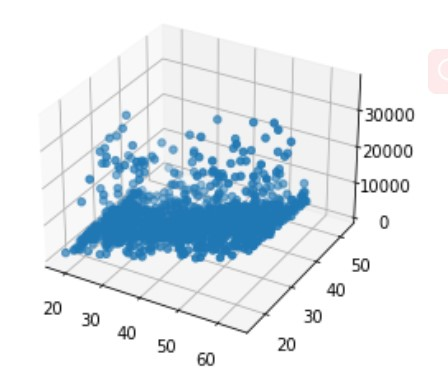
\includegraphics[width=6cm]{nonsmokeroverall.jpg}
\caption{Nonsmoker's condition}
\end{minipage}
\begin{minipage}[t]{0.48\textwidth}
\centering
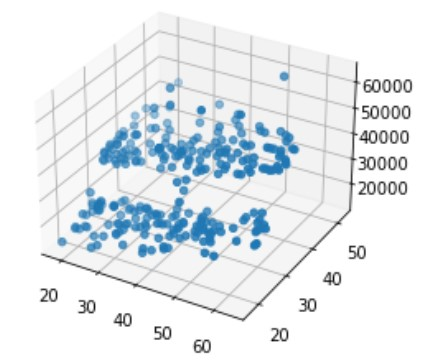
\includegraphics[width=6cm]{smokeroverall.jpg}
\caption{Smoker's condition}
\end{minipage}
\end{figure}

According to this observation, we are interested in whether it is reasonable to assume that the data in two labels are under different distributions. To examine this, we perform a hypothesis test on the mean of the two sets. 

\section{Clustering and Classification}
\subsection{Smokers' condition}

By observation of the BMI-charge(figure 3) and the age-charge(figure 4) figure, it is possible to separate the data from both graphs into two parts. 

\begin{figure}[H]
\centering
\begin{minipage}[t]{0.48\textwidth}
\centering
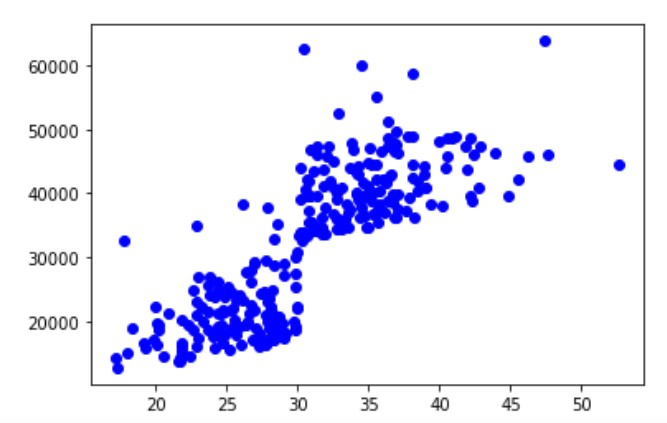
\includegraphics[width=6cm]{bmi-charge smoker.jpg}
\caption{BMI-charges figure}
\end{minipage}
\begin{minipage}[t]{0.48\textwidth}
\centering
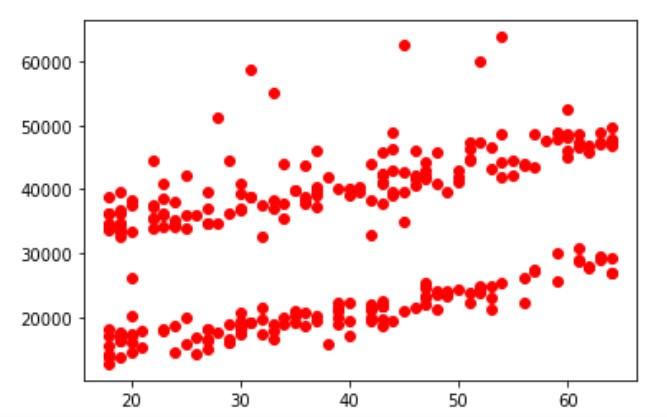
\includegraphics[width=6cm]{age-chargesmoker.jpg}
\caption{Age-charge figure}
\end{minipage}
\end{figure}


To do a more rigorous parting, Gaussian Mixture Model(GMM) is introduced to achieve this. For both graphs, the GMM model is set to do a two-cluster separation and achieves satisfying results as follows. As can be observed, even overlaying the two clustering together can almost separate the data points into two categories. One layer has obviously higher charges(over about 30,000) and higher BMI(over about 30) and the other's charges and BMI are lower.


\begin{figure}[H]
\centering
\begin{minipage}[t]{0.48\textwidth}
\centering
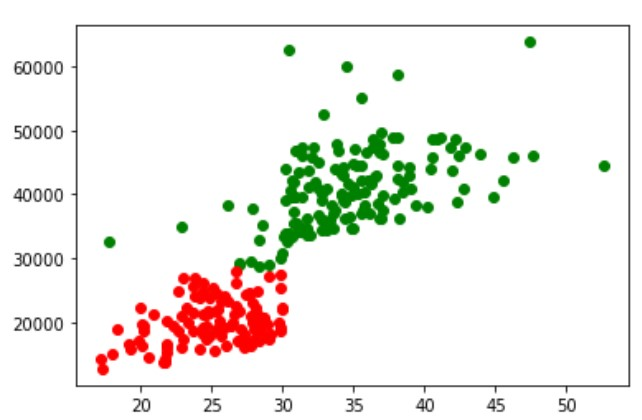
\includegraphics[width=6cm]{cluster result for bmi-charge.jpg}
\caption{clustering result for bmi-charge}
\end{minipage}
\begin{minipage}[t]{0.48\textwidth}
\centering
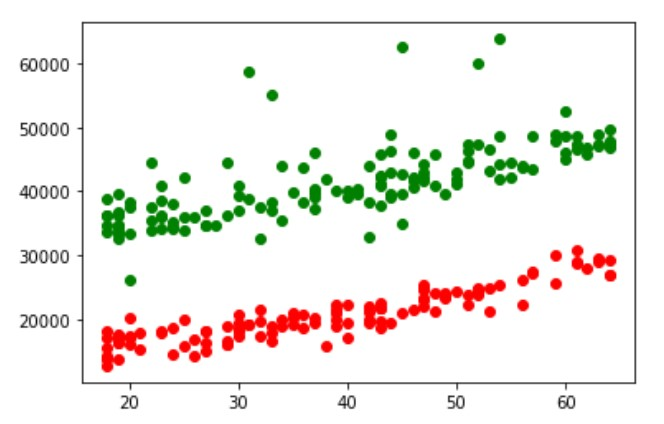
\includegraphics[width=6cm]{clustering result for age-charge.jpg}
\caption{clustering result for age-charge}
\end{minipage}
\end{figure}


According to the above analysis, the smoking population data can be divided into two categories: high charge and low charge. 
\begin{figure}[H]
\centering
\begin{minipage}[t]{0.48\textwidth}
\centering
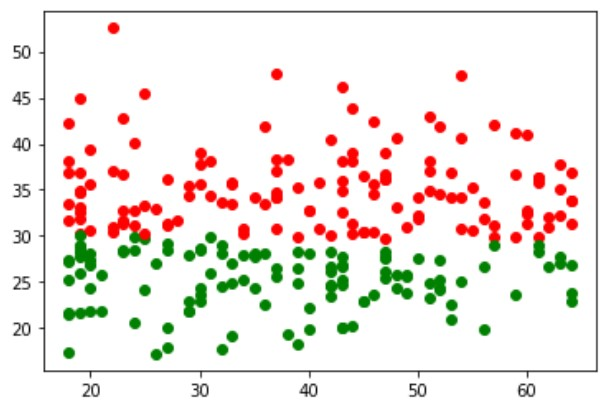
\includegraphics[width=6cm]{svm.jpg}
\caption{SVM Classification result}
\end{minipage}
\begin{minipage}[t]{0.48\textwidth}
\centering
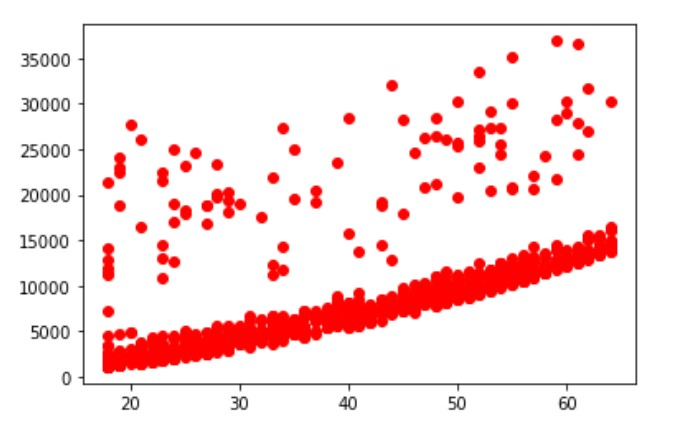
\includegraphics[width=6cm]{age-chargenonsmoker.jpg}
\caption{age-charge figure for non-smoker condition}
\end{minipage}
\end{figure}

\subsection{Non-smokers' condition}
By observation of the age-charges figure, The data are clustered densely in the low-charge area and scattered in the high-charge area. The GMM model is again used to cluster the data into two sets, whose result is in figure 9. The above clustering results projected onto age-bmi were shown in Figure 10, which is apparently terrible. Thus, the speculation is that we do not acquire enough data to perform a good classification among these data points. It may be caused by the lacking of customers with charges over 30000 but we do have not enough data to show. Consequently, what to be considered is merely cleaning the data by dropping out outliers and do not apply classification to the ‘non-smoker’ category afterward. 

\begin{figure}[H]
\centering
\begin{minipage}[t]{0.48\textwidth}
\centering
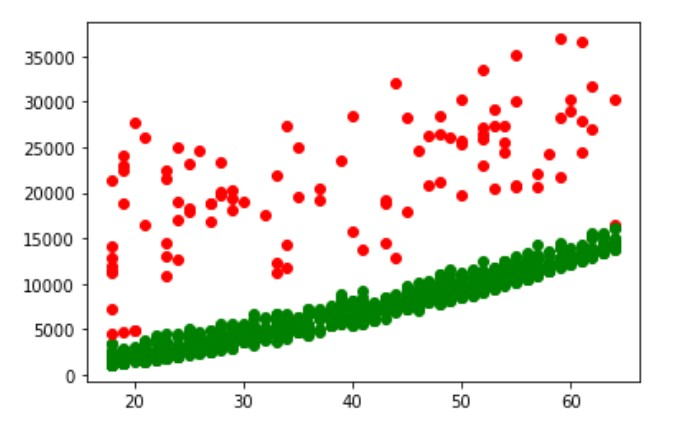
\includegraphics[width=6cm]{GMM RESULT with nonsmoker.jpg}
\caption{GMM result under nonsmoker condition}
\end{minipage}
\begin{minipage}[t]{0.48\textwidth}
\centering
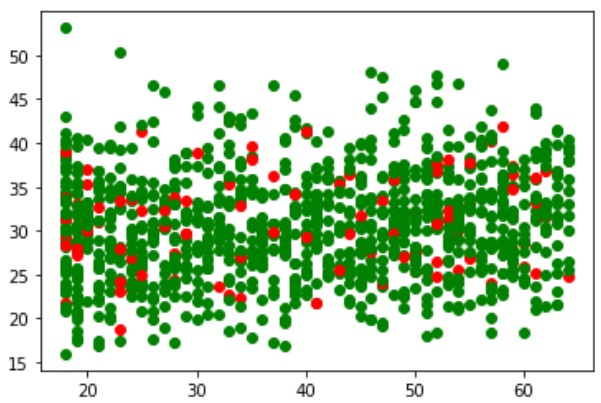
\includegraphics[width=6cm]{SVM2.jpg}
\caption{GMM cluster result on age bmi of non-smoker condition}
\end{minipage}
\end{figure}
In summary, currently, there are three categories, which are the nonsmoker category, the higher-charge smoker category, and the lower-charge smoker category.
\section{Linear Regression model}

\subsection{Simple Linear Regression with non-smoker category}
Consequently, Simple linear regression between age and charges is applied.
For input feature age (represented as X), the estimator for charges (represented as $\widehat{y}(x)$) can be calculated as:
$$\widehat{y}(x)=\widehat{\mu}_{Y \mid X=x}=\widehat{\beta}_{0}+\widehat{\beta}_{1} X $$,
The simple linear regression model from the R code is $Y = -3298.954 + 267.753x$, and $R^{2}$ is 0.8536, which is shown in figure 13.
Meanwhile, based on
$$\widehat{y}(x) \sim N\left(\mu_{Y \mid X=x}, \sigma^{2}\left(\frac{1}{n}+\frac{|x-\bar{x}|^{2}}{s_{x x}}\right)\right)$$
$$Y \mid(X=x)-\widehat{y}(x) \sim N\left(0, \sigma^{2}\left(1+\frac{1}{n}+\frac{|x-\bar{x}|^{2}}{s_{x x}}\right)\right)$$
With the unbiased estimator $s$ for $\sigma$, the  $0.95 $ confidence interval and the prediction interval are calculated and shown in figure 14.

\subsection{Multiple Linear Regression with higher-charges smokers category }
Firstly, the training set is also cleaned by means of controlling the standardized residual between -2 and 2.
Then, multiple linear regression is applied with the input features such as BMI and age, whose result is shown in figure 15. From the result, it is obvious that charges have almost no linear relationship with BMI, which shares the same conclusion as the Added-variable plot in figure 16. 

For input feature age (represented as $X_1$), the estimator for charges (represented as $\widehat{y}(x)$) can be calculated as:
$$\widehat{y}(x)=\widehat{\mu}_{Y \mid X=\vec{x} }=\widehat{\beta}_{0}+\widehat{\beta}_{1} X_1+ \widehat{\beta}_{2} X_2$$
The simple linear regression model from the R code is $Y = 13838.395 + 274.530 * X_1 + 463.828 * X_2$, and $R^{2}$ is  0.9027, which is shown in figure 15. The result is satisfying.
\subsection{Multiple Linear Regression with lower-charges smokers category}
Firstly, the training set is also cleaned by means of controlling the standardized residual between -2 and 2.
Then, multiple linear regression is applied with the input features such as BMI and age, whose result is shown in figure 17. From the result, it is obvious that charges have almost no linear relationship with BMI, which shares the same conclusion as the Added-variable plot in figure 18. 



The simple linear regression model from the R code is $Y =  67.902 + 258.458 * X_1 +  423.518 * X_2$, and $R^{2}$ is 0.9325, giving a desirable result which is shown in figure 15.

\section{Summary of techniques used that is not taught in class}

Gaussian Mixture Model is used to cluster the data and the Support Vector Machine is used to classify the data.
\section{Conclusion}
This paper focused on the relationship between 'charge' and its independent variables 'smoker', 'BMI', and 'age'. Our discussion is based on the fact that different 'smoker' labels would lead to a significant difference in the value of charges. Further experiments proved that 'smokers' can be parted into different classes for their charges with respect to 'age' and 'BMI', while 'non-smokers' does not produce such a separating effect so only one class is adopted in the result. Generally speaking, the charge of the above three classes all possess a strong positive linear relationship with age. 
The result shows that our model may produce more errors when predicting the non-smoker category. It is suggested that relevant data, e.g. family status, is lacking in the present model, and thus further research can be conducted with aims of observing the relation between family and charge.


\section{Appendix}
Data source: \\
\url{https://www.kaggle.com/datasets/mirichoi0218/insurance}\\
.csv version: \\
 \url{https://drive.google.com/file/d/1_VQk7_KoigrBS3NEPzBX5rdbI6CE4w43/view?usp=sharing}\\
Python Prepossessing code: \\
 \url{https://drive.google.com/file/d/1VziKPOPhUNzKtoHm06vYHopCrpNNXNq-/view?usp=sharing}

\end{document}
